\documentclass[a4paper,12pt]{article} % тип документа

% Поля страниц
\usepackage[left=2.5cm,right=2.5cm,
    top=2cm,bottom=2cm,bindingoffset=0cm]{geometry}
    
%Пакет дял таблиц   
\usepackage{multirow} 
    
%Отступ после заголовка    
\usepackage{indentfirst}


% Рисунки
\usepackage{floatrow,graphicx,calc}
\usepackage{wrapfig}

%%% Работа с картинками
\usepackage{graphicx}  % Для вставки рисунков
\graphicspath{{images/}{images2/}}  % папки с картинками
\setlength\fboxsep{3pt} % Отступ рамки \fbox{} от рисунка
\setlength\fboxrule{1pt} % Толщина линий рамки \fbox{}
\usepackage{wrapfig} % Обтекание рисунков и таблиц текстом

% Создаёем новый разделитель
\DeclareFloatSeparators{mysep}{\hspace{1cm}}

% Ссылки?
\usepackage{hyperref}
\usepackage[rgb]{xcolor}
\hypersetup{				% Гиперссылки
    colorlinks=true,       	% false: ссылки в рамках
	urlcolor=blue          % на URL
}


%  Русский язык
\usepackage[T2A]{fontenc}			% кодировка
\usepackage[utf8]{inputenc}			% кодировка исходного текста
\usepackage[english,russian]{babel}	% локализация и переносы

% Математика
\usepackage{amsmath,amsfonts,amssymb,amsthm,mathtools}

%%% Дополнительная работа с математикой
\usepackage{amsmath,amsfonts,amssymb,amsthm,mathtools} % AMS
\usepackage{icomma} % "Умная" запятая: $0,2$ $-$- число, $0, 2$ $-$- перечисление


% Что-то 
\usepackage{wasysym}


\begin{document}
\begin{center}
	\footnotesize{МОСКОВСКИЙ ФИЗИКО-ТЕХНИЧЕСКИЙ ИНСТИТУТ\\(НАЦИОНАЛЬНЫЙ 			ИССЛЕДОВАТЕЛЬСКИЙ УНИВЕРСИТЕТ)}\\
	\footnotesize{ФИЗТЕХ-ШКОЛА РАДИОТЕХНИКИ И КОМПЬЮТЕРНЫХ ТЕХНОЛОГИЙ\\}
	\hfill \break
	\hfill \break
	\hfill \break
	\hfill \break
	\hfill \break
	\hfill \break
\end{center}

\begin{center}   
    \hfill \break
	\hfill \break
	\hfill \break
	\hfill \break
	\hfill \break
	\hfill \break
	\hfill \break
	\hfill \break
	\hfill \break
	\hfill \break
	\hfill \break
	\large{Лабораторная работа № 4.3.1\\\large{\textbf{Изучение дифракции света}}}\\
	\hfill \break
        \hfill \break
	\hfill \break
	\hfill \break
	\hfill \break
	\hfill \break
	\hfill \break
	\hfill \break
	\hfill \break
	\hfill \break
	\hfill \break
	\begin{flushright}
		Климова Екатерина\\
		Группа Б01-108
	\end{flushright}
	\hfill \break
\end{center}
\hfill \break
\hfill \break
\begin{center}
	Долгопрудный, 2023 г.
\end{center}
\thispagestyle{empty}

\newpage
\hfill \break
\textbf{Цель работы:} исследовать явления дифракции Френеля и Фраунгофера на одной и двух щелях, изучить влияние дифракции на разрешающую способность оптических инструментов; проверить теоретические соотношения для положения максимумов при дифракции Френеля и Фраунгофера. 
\hfill \break
\hfill \break
\textbf{В работе используются:} оптическая скамья; ртутная лампа; светофильтр; щели с регулируемой шириной; рамка с вертикальной нитью; экран с двойной щелью; микроскоп на поперечных салазках с микрометрическим винтом; зрительная труба.

\section{Аннотация}
\hfill \break В первой части работы проводится исследование дифракции Френеля на узкой щели, на краю экрана, на тонкой нити; во второй части $ - $ дифракции Фраунгофера на щели и влияния изменения ширины щели и ее смещения на характер дифракционной картины. Далее рассматривается картина дифракции на двух щелях и оценивается влияние размеров источника на четкость картины. Наконец, в заключительной части работы проводится исследование влияния размера диафрагмы, ограничивающей поперечный размер пучка света, на четкость изображения объекта.

\section{Дифракция Френеля}
\subsection{Теоретические сведения и схема экспериментальной установки}

\begin{center}
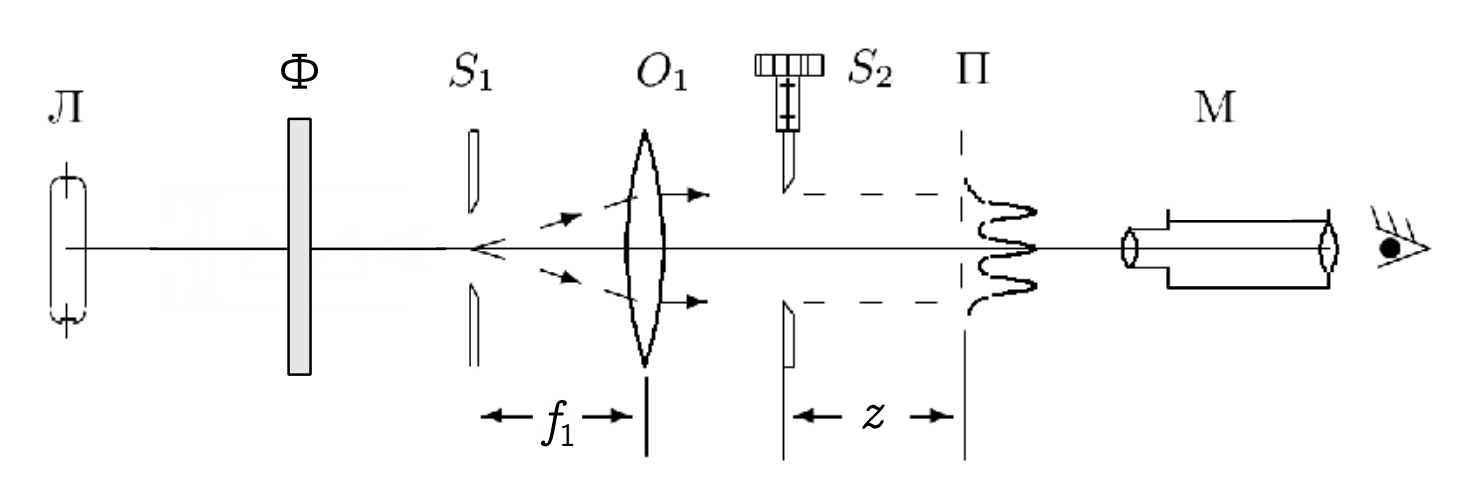
\includegraphics[width=0.75\textwidth]{4.3.1_1.png}\\
\textbf{Рис. 1.} Схема установки для наблюдения дифракции Френеля \\
\end{center}

\hfill \break Схема установки для наблюдения дифракции Френеля представлена на рис. 1. Свет от ртутной лампы Л, пропущенный через оранжевый светофильтр Ф со средней длиной волны $\lambda = 578$ нм, падает на входную щель $S_1$. Щель $S_1$ находится в фокусе \textit{коллиматора} $-$ собирающей линзы $O_1$. Коллиматор создает параллельный пучок монохроматического света, освещающий щель $S_2$, на которой и происходит дифракция. Дифракционная картина рассматривается с помощью микроскопа М, сфокусированного на некоторую плоскость наблюдения П.

\hfill \break Распределение интенсивности света в плоскости наблюдения П проще всего рассчитывать с помощью \textit{зон Френеля} (для щели их также называют \textit{зонами Шустера}). При освещении щели $S_2$ параллельным пучком лучей (плоская волна) зоны Френеля представляют собой полоски, параллельные краям щели (рис. 2). Результирующая амплитуда в точке наблюдения определяется суперпозицией колебаний от тех зон Френеля, которые не перекрыты створками щели. Границы зон Френеля/Шустера $\xi_m$ определяются соотношением

\begin{equation}\label{ linkname }
\xi_m = \pm \sqrt{mz\lambda}, \text{ } m \in \mathbb{N},
\end{equation}

\hfill \break где $\xi$ отсчитывается от центра щели, $z$ $-$ расстояние от щели до плоскости наблюдения П, а $\lambda$ $-$ длина волны. При ширине щели $b$ ($-b/2 < \xi < b/2$) полное число открытых зон для точки наблюдения на оси равно

$$
m_{\text{max}} = \frac{b^2}{4\lambda z}.
$$

\begin{wrapfigure}{l}{0.3\textwidth}
\begin{center}
    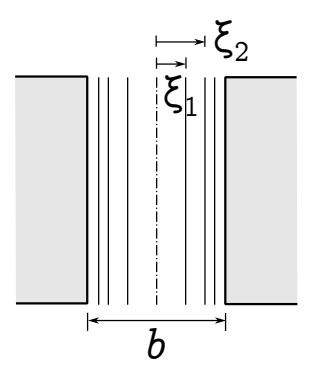
\includegraphics[width=1\textwidth]{4.3.1_2.png}
    \textbf{Рис. 2.} Зоны Шустера в плоскости щели
\end{center}
\end{wrapfigure}

\hfill \break По определению, разделение волнового фронта на зоны Френеля производится так, чтобы излучение от соседних зон находилось в противофазе. Иными словами, разность хода (от поверхности фронта до точки наблюдения) между краями соседних зон равна $\lambda/2$. Поэтому, когда открыто \textit{четное} число зон Френеля, на оси системы наблюдается \textit{минимум} дифракционной картины (темная полоса). Если число открытых зон \textit{нечетно}, в центре картины $-$ \textit{максимум} (светлая полоса).

\hfill \break Зафиксируем размер щели $b$ и проанализируем, как меняется картина в зависимости от расстояния до плоскости наблюдения $z$. Если число открытых зон Френеля велико, $m \gg 1$ $ (z \rightarrow 0)$, \textit{волновой параметр} $-$ $p = \frac{\lambda z} {b} \ll 1$, мы приходим к пределу геометрической оптики. В нем дифракционная картина отсутствует, а размер изображения щели совпадает с шириной самой щели $b$. Дифракционная картина наблюдается только в узкой полосе вблизи границ щели (<<дифракция на краю экрана>>). При удалении от плоскости геометрического изображения эти две группы полос постепенно расширяются, заполняя все изображение щели. При $m \sim 1$, $p \sim 1$ на щели наблюдается сложная картина из небольшого числа дифракционных полос. При дальнейшем удалении ($m \ll 1, \text{ } p \gg 1, \text{ } z \rightarrow \infty)$ дифракционная картина начинает упрощаться и расширяться, переходя в режим \textit{Фраунгофера} $-$ затухающие по интенсивности эквидистантные полосы с характерным угловым размером центральной полосы $\lambda / b$.

\hfill \break Амплитуду света в произвольной точке плоскости наблюдения можно определить графически с помощью векторной диаграммы $-$ \textit{спирали Корню}.

\hfill \break Распределение амплитуд в режиме дифракции Френеля ($m \sim 1$) довольно сложно. Однако если число открытых зон Френеля больше единицы и близко к целому $m = 2, \text{ } 3, \text{ } 4, \text{ } ...$ , то в картине можно довольно четко выделить $n = m - 1$ темных полос, заполняющих изображение щели. Так можно по виду дифракционной картины оценить число зон Френеля на полуширине щели. 

\subsection{Измерение и обработка результатов}
\hfill \break Для начала подготовим приборы к работе: настроим зрительную трубу на бесконечность, определим нуль микрометрического винта щели $S_2$, затем соберем схему согласно рис. 1. Линзу $O_1$ установим на расстоянии от $S_1$, близком к фокусному, которое указано на оправе линзы. При помощи зрительной трубы настроим пучок на бесконечность: поставим ее сразу за линзой $O_1$, убедимся, что пучок света проходит через центр линзы и попадает на центр объектива зрительной трубы; слегка перемещая линзу $O_1$ вдоль оси системы, найдем в окуляре зрительной трубы резкое изображение краев входной щели $S_1$. Щель $S_2$ поставим сразу за линзой и сфокусируем на ней микроскоп. При небольшом удалении микроскопа от щели на ярком фоне геометрического изображения появляются узкие темные дифракционные полосы, количество которых уменьшается по мере удаления микроскопа. Контрастность полученной картины зависит от ширины щели $S_1$ (при уменьшении щели растет контрастность, но падает яркость), от центрировки линзы, от равномерности освещения щелей и их параллельности.

\hfill \break Добившись наибольшей четкости и контрастности дифракционной картины, снова найдем резкое изображение щели (четкие края без дифракционных полос). Постепенно отодвигая микроскоп от щели $S_2$, заметим по шкале положение микроскопа, при котором на фоне щели видна одна темная полоса ($n = 1$). Смещение микроскопа от первоначального положения (от резкого изображения щели) дает величину $z$ $-$ расстояние от щели до плоскости наблюдения. 

\hfill \break Запишем ширину щели $S_2$: $b = (0.20 \pm 0.01)$ мм. Будем приближать микроскоп к щели, по мере этого снимем зависимость координаты микроскопа от числа $n = m - 1$ темных полос по формуле $a_{m} = x_{m} - x_{0}$, где  $x_{0} = 458$ мм $-$ начальное положение микроскопа (без дифракции). Из формулы (1), где $z = a_{m}$, найдем величину $2\xi_{m}$, при этом учтем, что длина волны зеленой линии ртути $\lambda = 5461 \cdot 10^{-10}$ м.

\begin{center}
\begin{tabular}{|c|c|c|c|c|}\hline
$ n $ & $ x_{m} $, мм & $ a_{m} $, мм & $ 2\xi_{m} $, мм & $ \sigma_{2\xi_{m}} $, мм\\\hline
1 & 474 & 16 & 0.17 & 0.01 \\\hline
2 & 467 & 9 & 0.20 & 0.01 \\\hline
3 & 464 & 6 & 0.20 & 0.01 \\\hline
4 & 462 & 4 & 0.19 & 0.01 \\\hline
5 & 461 & 3 & 0.18 & 0.01 \\\hline
\end{tabular} \\
\hfill \break \textbf {Таблица 1.} Зависимость координаты микроскопа от числа зон Френеля на полуширине щели\\
\end{center}

\hfill \break Погрешность $\sigma_{x_m} = 0.5$ мм получается из половины цены деления поперечных салазок микроскопа. Рассчитаем погрешность измерения $2\xi_{m}$ путем почленного дифференцирования формулы (1):

$$
\sigma_{2\xi_m} = 2\xi_{m} \cdot \sqrt{ \left( \frac{ \partial (2 \sqrt{ a_{m}m \lambda} } { \partial a_{m}} \right)^2 \sigma_{a_m}^2 } = 2z_{m} \sqrt{ \frac{ m \lambda} {a_{m}} } \sigma_{a_{m}}.
$$

\hfill \break Учитывая, что $\xi_{m} = \sqrt{ a_{m} m\lambda}$, получим, что $\sigma_{2\xi_{m}} = 2m\lambda \sigma_{a_{m}}$. Усреднив $2\xi_{m}$, получим ширину щели $b$, погрешность для которой можно рассчитать как

$$
\sigma_{b_{\text{ср}}} = \frac {1} {\sqrt{ n (n-1) }} \cdot \sqrt {\sum_{i=1}^{n} (b_{i} - b_{\text{ср}})^2}.
$$

\hfill \break По полученным данным построим график вида $2\xi_{m} = f(m)$, где $m = n + 1$:

\begin{center}
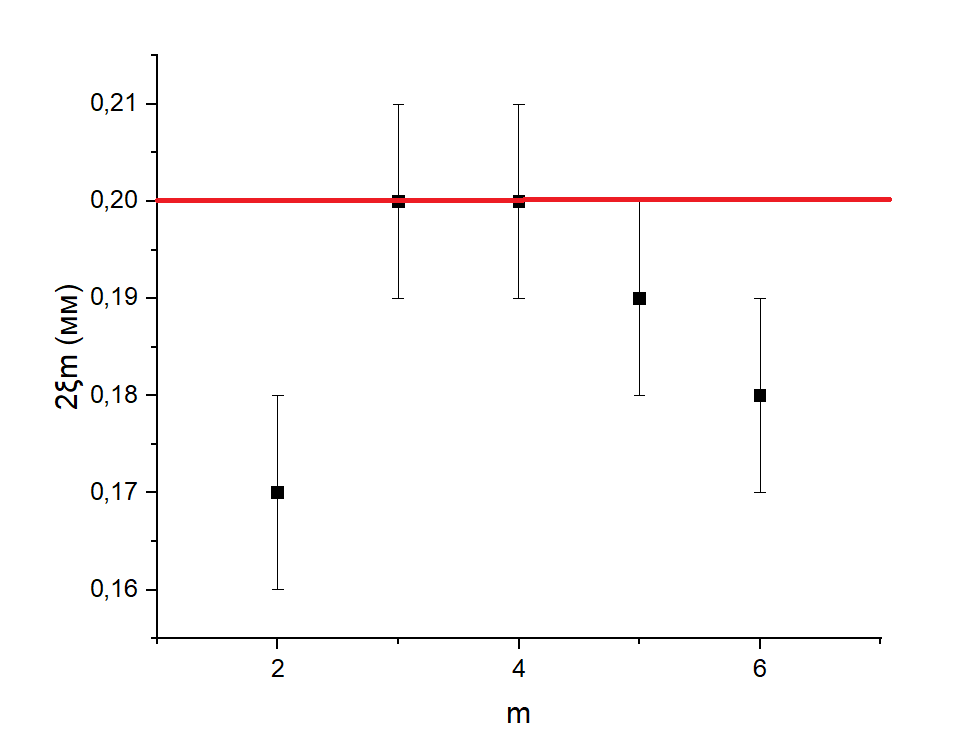
\includegraphics[width=0.65\textwidth]{4.3.1_3.png}\\
\textbf{Рис. 3.} График зависимости ширины щели $S_2$ от числа открытых зон Френеля \\
\end{center}

\hfill \break Красной линией на графике отмечено измеренное ранее значение ширины щели $b$. Экспериментально полученное значение равно $b_{\text{эксп}} = (0.19 \pm 0.01)$ мм, что отлично сходится с измеренным значением в пределах погрешности.

\hfill \break При уменьшении щели уменьшается количество дифракционных полос, что согласуется с теорией и обусловлено возрастанием волнового параметра. 

\section{Дифракция Фраунгофера на щели}
\subsection{Теоретические сведения и схема экспериментальной установки}

\hfill \break На значительном удалении от щели, когда выполнено условие $m \ll 1$ (то есть ширина щели становится значительно меньше ширины первой зоны Френеля, $b \ll \sqrt{\lambda z}$), изображение щели размывается и возникает дифракционная картина, называемая \textit{дифракцией Фраунгофера}.

\hfill \break Дифракцию Фраунгофера можно наблюдать на той же установке, что и дифракцию Френеля (рис. 1). Однако при обычных размерах установки дифракция Фраунгофера возникает только при очень узких щелях. Поскольку работать с тонкими щелями неудобно, для наблюдения дифракции Фраунгофера к схеме добавляется объектив $O_2$ (рис. 4):

\begin{center}
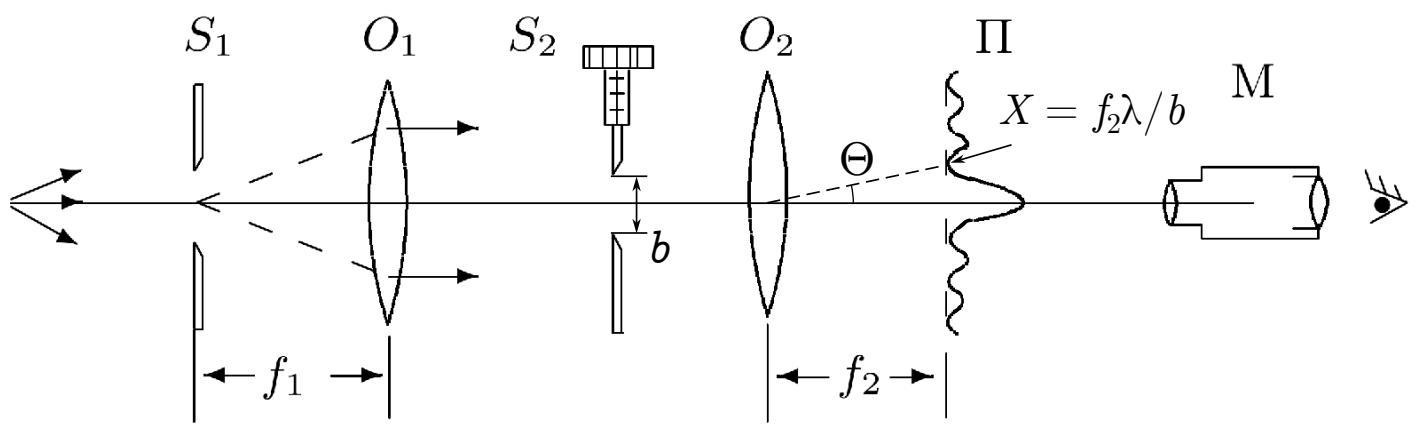
\includegraphics[width=0.75\textwidth]{4.3.1_4.png}\\
\textbf{Рис. 4.} Схема установки для наблюдения дифракции Фраунгофера на щели \\
\end{center}

\hfill \break Дифракционная картина наблюдается в фокальной плоскости объектива $O_2$. Поскольку объектив не вносит дополнительной разности хода между интерферирующими лучами (\textit{таутохронизм} тонкой линзы), в его фокальной плоскости наблюдается неискаженная дифракционная картина Фраунгофера, соответствующая бесконечно удаленной плоскости наблюдения.

\hfill \break При дифракции Фраунгофера в центре поля зрения наблюдается дифракционный максимум (светлая полоса). Сбоку от нее наблюдаются чередующиеся минимумы и максимумы с довольно быстро затухающей интенсивностью. Направление на минимумы (темные полосы) при малых углах $\Theta$ определяется соотношением

\begin{equation}\label{ linkname }
\Theta_{n}^{\text{min}} = n\frac{\lambda}{b}, \text{ } n = \pm 1, \text{ }, \pm 2, \text{ } ... \text{ },
\end{equation}

\hfill \break где $b$ $-$ ширина щели. Каждому значению угла $\Theta$ соответствует точка в плоскости объектива с фокусным расстоянием $f_{2}$, отстоящая от оптической оси на расстоянии

\begin{equation}\label{ linkname }
X_{n} = f_2 \tg {\Theta_{n}} \approx f_2 \Theta_{n}.
\end{equation}

\hfill \break Измеряя зависимость $X$ от $n$ или расстояние между полосами $\Delta X$, можно определить ширину щели $S_2$.

\subsection{Измерение и обработка результатов}

\hfill \break Соберем схему в соответствии с рис. 4. Настроим микроскоп на фокальную плоскость П линзы. Для этого временно снимем со скамьи щель $S_2$ и убедимся, что свет проходит через центры линз и попадает на объектив микроскопа. Перемещая микроскоп вдоль скамьи, найдем резкое изображение щели $S_1$. Закрепим микроскоп и линзы на скамье.

\hfill \break Вернем щель $S_2$ на ее место между линзами и подберем ширину так, чтобы в поле зрения микроскопа появилась дифракционная картина. В отличие от френелевой дифракционной картины, фраунгоферова занимает все поле зрения микроскопа. Уменьшая ширину входной щели $S_1$, добьемся наибольшей контрастности картины.

\hfill \break Зафиксируем величину щели $S_2$ по микрометрическому винту $b = (0.32 \pm 0.01)$ мм и фокусное расстояние линзы $f_2 = 12.5$ см. 

\hfill \break Измерим с помощью окулярной шкалы микроскопа координаты $x_{n}$ нескольких дифракционных минимумов в обе стороны от центра. Результаты измерений занесем в таблицу:

\begin{center}
\begin{tabular}{|c|c|c|c|c|c|c|c|c|}\hline
$ n $ & $ -3 $ & $ -2 $ & $ -1 $ & $ 0 $ & $ 1 $ & $ 2 $ & $ 3 $ & $ 4 $ \\\hline
$ x_{n} $, мм & $ 1.12 $ & $ 1.13 $ & $ 1.50 $ & $ 1.71 $ & $ 1.92 $ & $ 2.08 $ & $ 2.26 $ & $ 2.46 $ \\\hline
\end{tabular} \\
\hfill \break \textbf {Таблица 2.} Координаты дифракционных минимумов \\
\end{center}

\hfill \break Построим график зависимости экстремумов $x_{n}$ дифракционной картины от их номеров $n$, убедимся, что она может быть аппроксимирована прямой линией:

\begin{center}
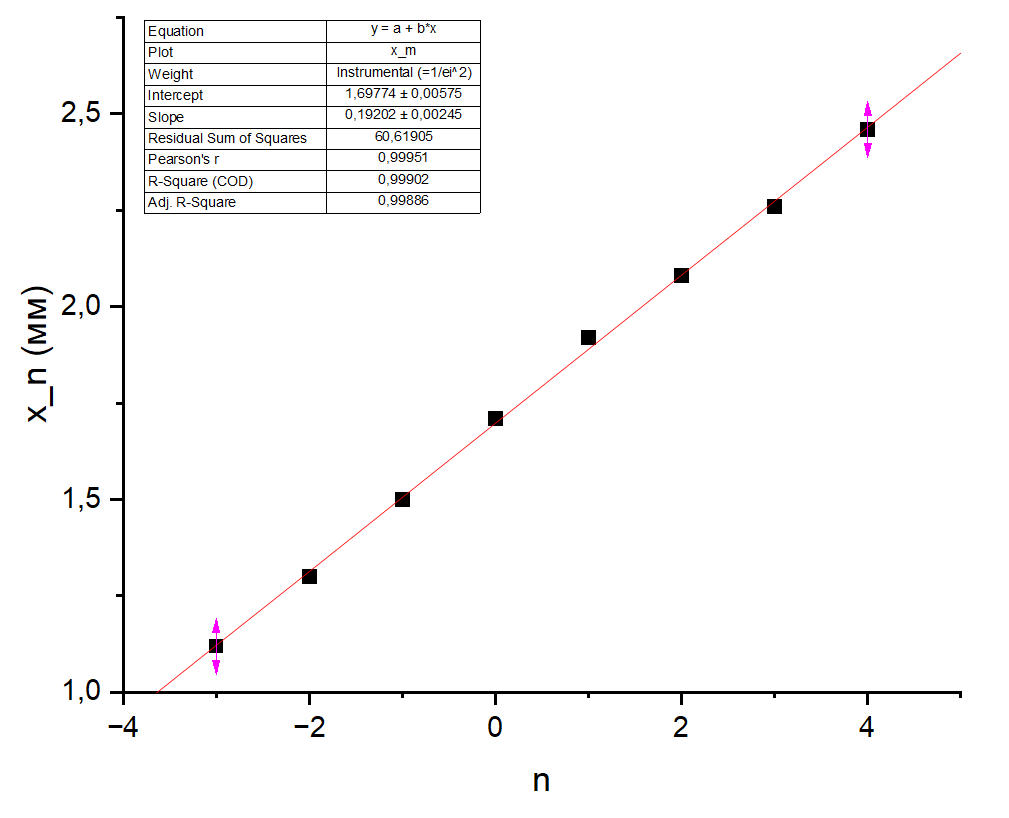
\includegraphics[width=0.75\textwidth]{4.3.1_5.png}\\
\textbf{Рис. 5.} График зависимости экстремумов дифракционной картины от их номеров \\
\end{center}

\hfill \break По углу наклона графика определим среднее расстояние $\Delta X = (19.20 \pm 0.25) \cdot 10^{-2}$ мм; по формуле (3) рассчитаем ширину щели $b = \frac {\lambda} {\Delta X} f_2 = (35.5 \pm 4.6) \cdot 10^{-2}$ мм, что очень близко к измеренному значению.  

\hfill \break Коэффициент наклона графика и погрешность его расчета мы определили из МНК: 

$$
k = \frac {<xy>} {x^2}, \text{ } \sigma_{k} \approx \frac{1} {\sqrt{n}} \sqrt{ \frac {<y^2>} {x^2} - k^2}.
$$

\hfill \break Наконец, убедимся, что смещение щели $S_2$ в боковом направлении не приводит к сдвигу дифракционной картины. Это свяазано с тем, что картина находится в фокальной плоскости линзы $O_2$, куда приходят почти параллельные лучи. При уменьшении ширины щели картина растягивается, пока полностью не исчезнет, что согласуется с формулой (3). 

\section{Дифракция Фраунгофера на двух щелях}
\subsection{Теоретические сведения и схема экспериментальной установки}

\hfill \break Схема для наблюдения дифракции Фраунгофера на двух щелях изображена на рис. 6. По сравнению с рис. 4 в ней щель $S_2$ заменена на экран Э с двумя щелями. При этом щель $S_2$ (с микрометрическим винтом) установлена вместо входной щели $S_1$ (для измерения влияния ширины источника на четкость картины). 

\hfill \break Результат дифракции на двух щелях можно представить как \textit{интерференцию} дифракционных картин от каждой щели (аналог интерференционной схемы Юнга).

\begin{center}
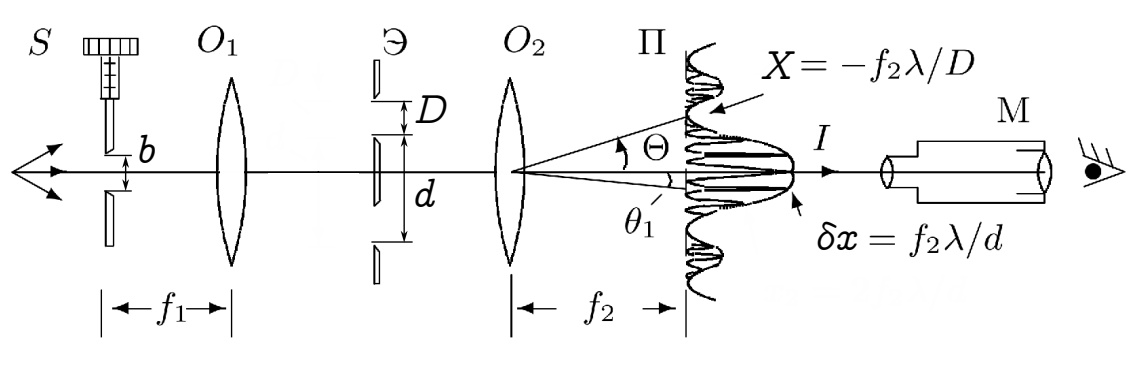
\includegraphics[width=0.75\textwidth]{4.3.1_6.png}\\
\textbf{Рис. 6.} Схема установки для наблюдения дифракции Фраунгофера на двух щелях \\
\end{center}

\hfill \break Если входная щель достаточно узка, то дифракционная картина в плоскости П (рис. 6) подобна той, что получалась при дифракции на одной щели, однако теперь вся картина испещрена рядом дополнительных узких полос. Наличие этих полос объясняется суперпозицией (интерференцией) световых волн, приходяших в плоскость наблюдения через разные щели экрана Э. В центре главного дифракционного максимума располагается светлая полоса (разность на оси, в силу симметрии, равна нулю). Светлая интерференционная полоса наблюдается также, когда разность хода кратна длине волны. Угловая координата $\Theta_n$ интерференционного максимума $n$-го порядка определяется соотношением

\begin{equation}\label{ linkname }
\Theta_n d = n\lambda, n = \pm 1, \text{ } \pm 2, \text{ } ... \text{ },
\end{equation}

\hfill \break где $d$ $-$ расстояние между щелями. Линейное расстояние $\delta x$ между соседними интерференционными полосами в плоскости П равно поэтому

\begin{equation}\label{ linkname }
\delta x = f_2 \frac {\lambda} {d}.
\end{equation}

\hfill \break На рис. 4 показано распределение интенсивности в фокальной плоскости объектива $O_2$. Штриховой линией (в увеличенном масштабе) изображено распределение интенсивности при дифракции света на одиночной щели. Поскольку полная угловая ширина главного дифракционного максимума (от минимума до минимума) равна $2\lambda/D$, где $D$ $-$ ширина отдельной щели, то на нем укладывается $N = \frac {2d} {D}$ \textit{темных} интерференционных полос (в центре картины максимум, поэтому светлых полос $-$ на одну больше).

\hfill \break При дифракции света на двух щелях четкая система интерференционных полос наблюдается только при достаточно узкой ширине входной щели $S_2$, которую можно рассматривать как протяженный источник света размером $b$. Для наблюдения интерференции необходимо, чтобы расстояние $d$ между щелями не превышало \textit{радиуса когерентности}:

\begin{equation}\label{ linkname }
d \le \rho_{\text{ког}} \approx \frac{\lambda}{b} f_1.
\end{equation}

\hfill \break Таким образом, по размытию интерференционной картины можно оценить размер источника $b$. Этот метод используется в звездном интерферометре при измерении угловых размеров звезд.

\subsection{Измерение и обработка результатов}

\hfill \break Не перемещая линз и микроскопа в уже собранной установке, уберем входную щель $S_1$ и установим на ее место щель с микрометрическим винтом $S_2$. Слегка передвигая щель $S_2$ вдоль скамьи, найдем в микроскопе резкое изображение новой входной щели. Закрепим щель.

\hfill \break Поставим между линзами (там, где раньше была щель $S_2$) экран Э с двойной щелью. В области главного дифракционного максимума появилась система равноотстоящих темных и светлых полос. Центрировкой системы и подбором ширины входной щели добьемся наибольшей четкости дифракционной картины. 

\hfill \break Проведем измерения и расчеты, результаты которых представим в таблице:

\begin{center}
\begin{tabular}{|c|c|c|c|c|}\hline
$ N $ & $ X $, $10^{-2}$ мм & $ \delta x $, $ 10^{-2} $ мм & $ d $, $ 10^{-2}$ мм & $ D $, $ 10^{-2} $ мм \\\hline
$ 9 $ & $ 68 \pm 1 $ & $ 7.6 \pm 0.1 $ & $ 90.3 \pm 1.8 $ & $ 20.1 \pm 0.4 $ \\\hline
\end{tabular} \\
\hfill \break \textbf {Таблица 3.} Измерения и расчеты \\
\end{center}

\hfill \break Здесь $N$ $-$ число темных интерференционных полос внутри главного максимума, $X$ $-$ ширина главного максимума, $\delta x = X/N$ $-$ линейное расстояние между соседними интерференционными полосами, $d = f_2 \lambda / \delta x$ $-$ расстояние между щелями, $D = 2d/N$ $-$ ширина щели.

\hfill \break Также при помощи микроскопа измерим ширину двойных щелей $D = (0.20 \pm 0.02)$ мм и расстояние между ними $d = (0.92 \pm 0.02)$ мм. При этом погрешность:
$$
\sigma_{d} = d \cdot \sqrt{ \left( \frac { \partial \left( f_2 \frac {\lambda} {\delta x} \right)} { \partial (\delta x) } \right)^2 \cdot \sigma_{\delta x}^2} = d \cdot f_2 \lambda \frac{1} {\delta x^2} \cdot \sigma_{\delta x},
$$

$$
\Rightarrow \sigma_{d} = \frac{d^2}{\delta x} \sigma_{\delta x}.
$$

\section{Влияние дифракции на разрешающую способность оптического инструмента}
\subsection{Теоретические сведения и схема экспериментальной установки}

\hfill \break Установка (рис. 7) позволяет исследовать влияние дифракции на \textit{разрешающую способность} оптических инструментов. 

\hfill \break Линзы $O_1$ и $O_2$ (без щели $S_2$) создают в плоскости П изображение щели входной $S_1$, рассматриваемое в микроскоп М. Таким образом, пара линз $O_1$ и $O_2$ и микроскоп в совокупности могут рассматриваться как некий \textit{оптический инструмент}. При этом входная щель $S_1$ и коллиматор $O_1$ создают модель далекого предмета, а объектив $O_2$ и микроскоп М составляют <<зрительную трубу>>, наведенную на этот предмет.

\hfill \break Если перед объективом $O_2$ зрительной трубы расположить щель $S_2$, то изображение объекта будет \textit{искажено дифракцией} на щели $S_2$. Чем меньше ширина $b$ этой щели, тем сильнее искажение. Качественной характеристикой этих искажений может служить минимальное угловое расстояние $\varphi$ между точками рассматриваемого предмета, которые воспринимаются как раздельные.

\begin{center}
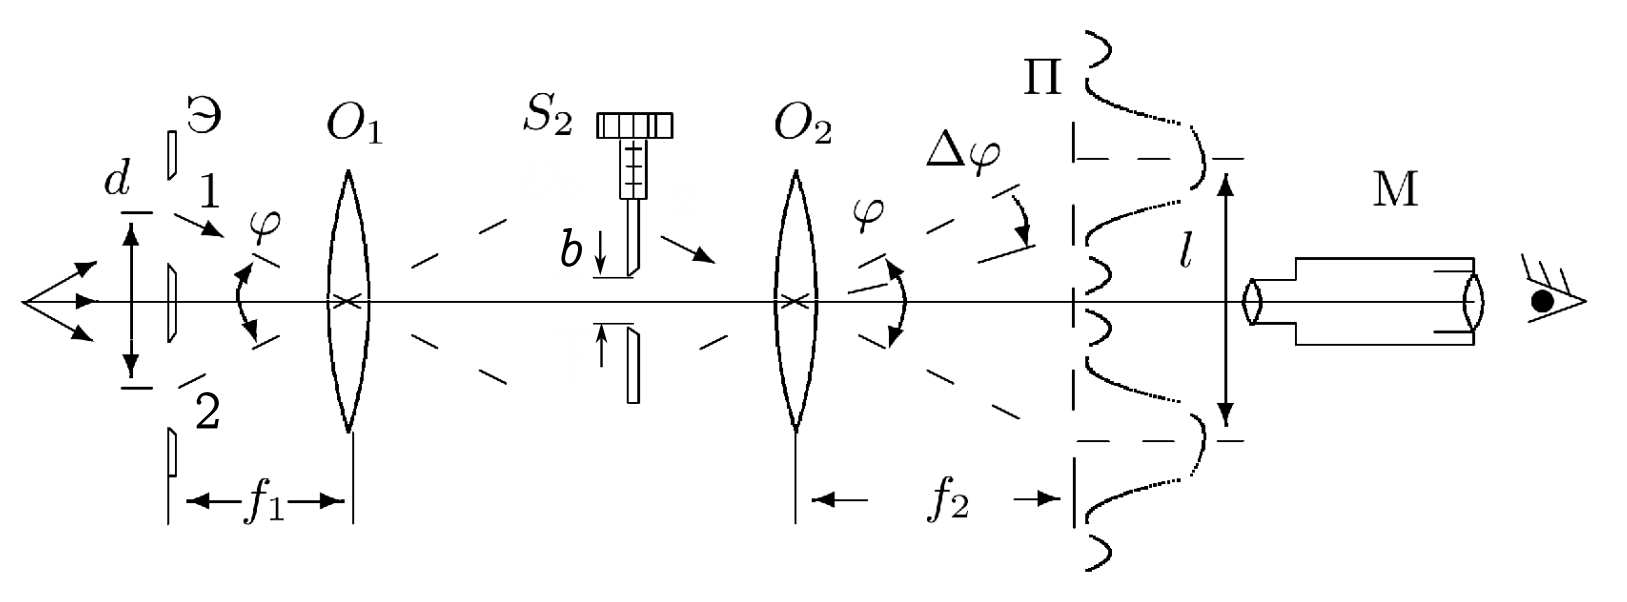
\includegraphics[width=0.75\textwidth]{4.3.1_7.png}\\
\textbf{Рис. 7.} Схема установки для исследования разрешающей способности оптического инструмента \\
\end{center}

\hfill \break В качестве предмета будем использовать экран Э с двумя узкими щелями (поместим его вместо $S_1$). Пусть расстояние между щелями равно $d$. Тогда от каждой из щелей экрана на щель $S_2$ будут падать два параллельных пучка света, составляющих между собой угол 

\begin{equation}\label{ linkname }
\varphi \approx \frac {d} {f_1}
\end{equation}

\hfill \break (а центры двух дифракционных пятен в плоскости П будут находиться на расстоянии $l = f_2 \varphi$ друг от друга).

\hfill \break Угловая ширина же $\Delta \varphi$ каждого изображения определяется \textit{дифракцией} света на щели $S_{2}$. В режиме дифракции Фраунгофера полуширина центрального дифракционного максимума равна $\Delta \varphi \sim \lambda / b$, где $b$ $-$ ширина щели $S_2$.

\hfill \break Если полуширина главного дифракционного пятна превысит расстояние между центрами пятен $\Delta \varphi > \varphi$, пятна от двух щелей сольются в одно и по виду дифракционной картины будет трудно определить, представляет ли собой источник двойную или одиночную щель. Это условие разрешения двух изображений называется \textit{критерием Рэлея}. Итак, щели можно считать различимыми, если 

\begin{equation}\label{ linkname }
\frac {\lambda} {b} < \frac {d} {f_1}.
\end{equation}

\subsection{Измерение и обработка результатов}
\hfill \break Соберем схему согласно рис. 7. Для этого в предыдущей схеме, не меняя положений линз и микроскопа, уберем входную щель и поставим на ее место экран с двойной щелью. Перемещая экран вдоль оси системы, получим в поле зрения микроскопа четкое симметричное изображение двойного источника. Установим максимальную ширину щели $S_2$ и поставим ее между линзами $O_1$ и $O_2$. Постепенно уменьшая ее ширину $b$, пронаблюдаем за ухудшением качества изображения двойной щели в микроскоп. 

\hfill \break Подберем ширину $b_0$ щели $S_2$ так, чтобы изображения обеих щелей почти сливались, но все-таки воспринимались отдельно. Для проверки разрешающей способности по критерию Рэлея сравним измеренную ширину $b_0$ щели $S_2$ с расчетом по формуле (8):

\begin{center}
\begin{tabular}{|c|c|}\hline
$ b_{0} $, $10^{-2}$ мм & $ \lambda f_1 /d $, $10^{-2}$ мм \\\hline
$ 27.3 $ & $ 6.0 $ \\\hline
\end{tabular} \\
\hfill \break \textbf {Таблица 4.} Сравнение измеренного и рассчитанного значений \\
\end{center}

\section{Вывод}
\hfill \break Мы изучили два основных вида дифракции: Френеля и Фраунгофера при различных размерах щели и экспериментально проверили справедливость теоретических формул. 

\hfill \break \textbf{Дифракция Френеля.} По результатам измерений и проведённых вычислений можно утверждать, что полученная ширина щели примерно одинакова и совпадает с результатом, измеренным микрометрическим винтом в пределах погрешности. Некоторые отличия результата от цели можно связать с неточностью определения <<сдвига>> микроскопа и нуля микрометрического винта. 

\hfill \break Кроме того, при дифракции на препятствии при удалении микроскопа от нити на её фоне всегда наблюдали чётное число тёмных дифракционных полос и светлый центр.

\hfill \break \textbf{Дифракция Фраунгофера на одной щели.} Значение для ширины щели
$$
\boxed{b =  (35.5 \pm 4.6) \cdot 10^{-2} \; \text{мм},} 
$$
\hfill \break вычисленное по формуле, совпадает в пределах погрешности с величиной, измеренной по микрометрической шкале:
$$
\boxed{b =  (32.0 \pm 1.0) \cdot 10^{-2} \; \text{мм}.} 
$$
\hfill \break Это подтверждает теоретические выкладки и говорит о выполнении предложенной теории.

\hfill \break \textbf{Дифракция Фраунгофера на двух щелях.} Измеренные экспериментально ширина щели и расстояние между щелями совпадают с измеренными <<напрямую>>.

\[ \boxed{d_\text{экс} = (0.90 \pm 0.02) \text{ мм},} \]
\[ \boxed{D_\text{экс} = (0.20 \pm 0.01) \text{ мм},} \]
\[ \boxed{d_\text{микр} = (0.92 \pm 0.02) \text{ мм},} \]
\[ \boxed{D_\text{микр} = (0.20 \pm 0.02) \text{ мм}.} \]

\hfill \break \textbf{Влияние дифракции на разрешающую способность оптического инструмента}. В результате измерений получаем, что $b_0 > \lambda f_1/d$, что означает разрешимость изображений по Рэлею, что мы и наблюдали в ходе выполнения работы.

\hfill \break \textbf{Общие выводы}. Полученные в ходе выполнения работы результаты подтверждают теоретические сведения. Все результаты с неплохой точностью сошлись с <<целевыми>> показателями, они совпали в пределах погрешностей. Основной вклад в них могли внести аберрации света, которые могли возникнуть из-за недостаточно точной настройки оптической системы для выполнения работы. Также свой вклад вносит неточность определения линейных размеров объектов при помощи микроскопа, особенно при определении координат дифракционных максимумов. Кроме того, неточность вносит некоторая неопределённость при установлении положения нуля зазора $ S_2 $.

\end{document}
